%This is the fourth chapter of the dissertation

%The following command starts your chapter. If you want different titles used in your ToC and at the top of the page throughout the chapter, you can specify those values here. Since Columbia doesn't want extra information in the headers and footers, the "Top of Page Title" value won't actually appear.

\pagestyle{cu}
\graphicspath{{./Chapter4/Figures/}}
\chapter[Purity and the Electron Lifetime][Purity and the Electron Lifetime]{Purity and the Electron Lifetime}

In a noble element dark matter detection experiment the purity of the target mass is an essential consideration and must be measured
continuously.  To date the concentration of electronegative impurities has always been measured in these experiments, but no reliable
model has existed to explain and predict its behavior.

In this chapter I discuss the necessity of extremely pure xenon (\secref{}), explain the original model fit to XENON1T data
(\secref{}), and examine how abrupt changes in detector conditions alter the contamination (\secref{}).



\section{Importance and Procedure for Purifying Xenon}
\secref{sec:importance_procedure}
Purity usually refers to two distinct but correlated values, though the degree of the correlation can depend on the
experiment.  The first is radioactive elements of other noble elements that cannot be completely removed during distillation.  For xenon
our primary challenges are \ce{^{85}Kr} (\secref{subsubsec:backgrounds_electronic_krypton}) and \ce{^{222}Rn}
(\secref{subsubsec:backgrounds_electronic_radon}) as they have low-energy decays that can contaminate our region of interest (while
\ce{^{220}Rn} also leads to a low-energy \betadecay its half-life is too short to penetrate our detector and thus can be ignored).

The second consideration with regards to detector purity is contamination of electronegative impurities such as \ce{O_2} or
\ce{N_2}.  These attach to drifting electrons, lowering or even eliminating the S2.  This can have the largest impact at low energies
since the number of \electron is much fewer.  To correct for the expected initial number of electrons we can use the electron lifetime
$\tau_{\mathrm{e^-}}$, though this must be monitored consistently if not perpetually.  Of course, if the entire cloud of electrons is
removed by these impurities we cannot apply a correction since we have no knowledge of where in the detector it occurred or the energy
deposition.

This chapter is focused on the latter of these two purities, though its examination necessitates consideration of the former as we will
see.



\section{Effects of Electronegative Impurities}
\label{sec:importance_procedure_effects}
Impurities mainly come from outgassing of detector materials and diffusion of elements in the air surrounding the detector through seals,
though for the latter this is primarily limited to noble gases such as \ce{^{222}Rn} (\textbf{check this}).  While many of these
contribute to our electronic recoil background (\secref{subsec:backgrounds_electronic}) they can also decrease the number of photons and
electrons measured.

\subection{Photon Attenuation}
\label{subsec:importance_procedure_effects_photons}
Contaminants been shown to absorb Xe scintillation (178 nm with ${\sim} 14\ \mathrm{nm}$ spectral FWHM)
(\citeref{Watanabe1953a, Watanabe1953b}).  At concentrations of ppm or higher
the fraction of UV photons that reach the PMTs can be considerably decreased - especially for large detectors.  The intensity due to
photon attenuation is given by

\begin{equation}
I(x) = I_0 e^{-x / \lambda_{\mathrm{att}}}
\end{equation}

\nonindent where $I_0$ is initial intensity, $x$ is distance, and $\lambda_{\mathrm{att}}$ is the attenuation length.  It can be written
as $1 / \lambda_{\mathrm{att}} = 1 / \lambda_{\mathrm{abs}} + 1 / \lambda_{\mathrm{scatt}}$ where $\lambda_{\mathrm{abs}}$ and
$\lambda_{\mathrm{scatt}}$ are the the absorption and scatterings lengths, respectively.  For entirely pure xenon
$\lambda_{\mathrm{abs}} \sim \infty$ (\citeref{Baldini2005} found $lambda_{\mathrm{abs}} > 100\ \mathrm{cm}$ at 90\% confidence
level).

The inclusion of impurities, however, can shorten the absorption
length.  \figerf{fig:importance_procedure_effects_photons_absorption_coefficents} shows the absorption coefficients
($\lambda_{\mathrm{abs}}^{-1}$) for 1 ppm \htwoo and \otwo from $130 \mdash 200\ \mathrm{nm}$.  They overlap with shorter wavelengths
of the xenon spectrum (included for comparison), meaning measured VUV photons by PMTs will not be symmetric above 178 nm.  With a nearly
1-meter tall detector a 1 ppm concentration of \htwoo would have an effect at 184 nm.

\begin{figure}
\centering
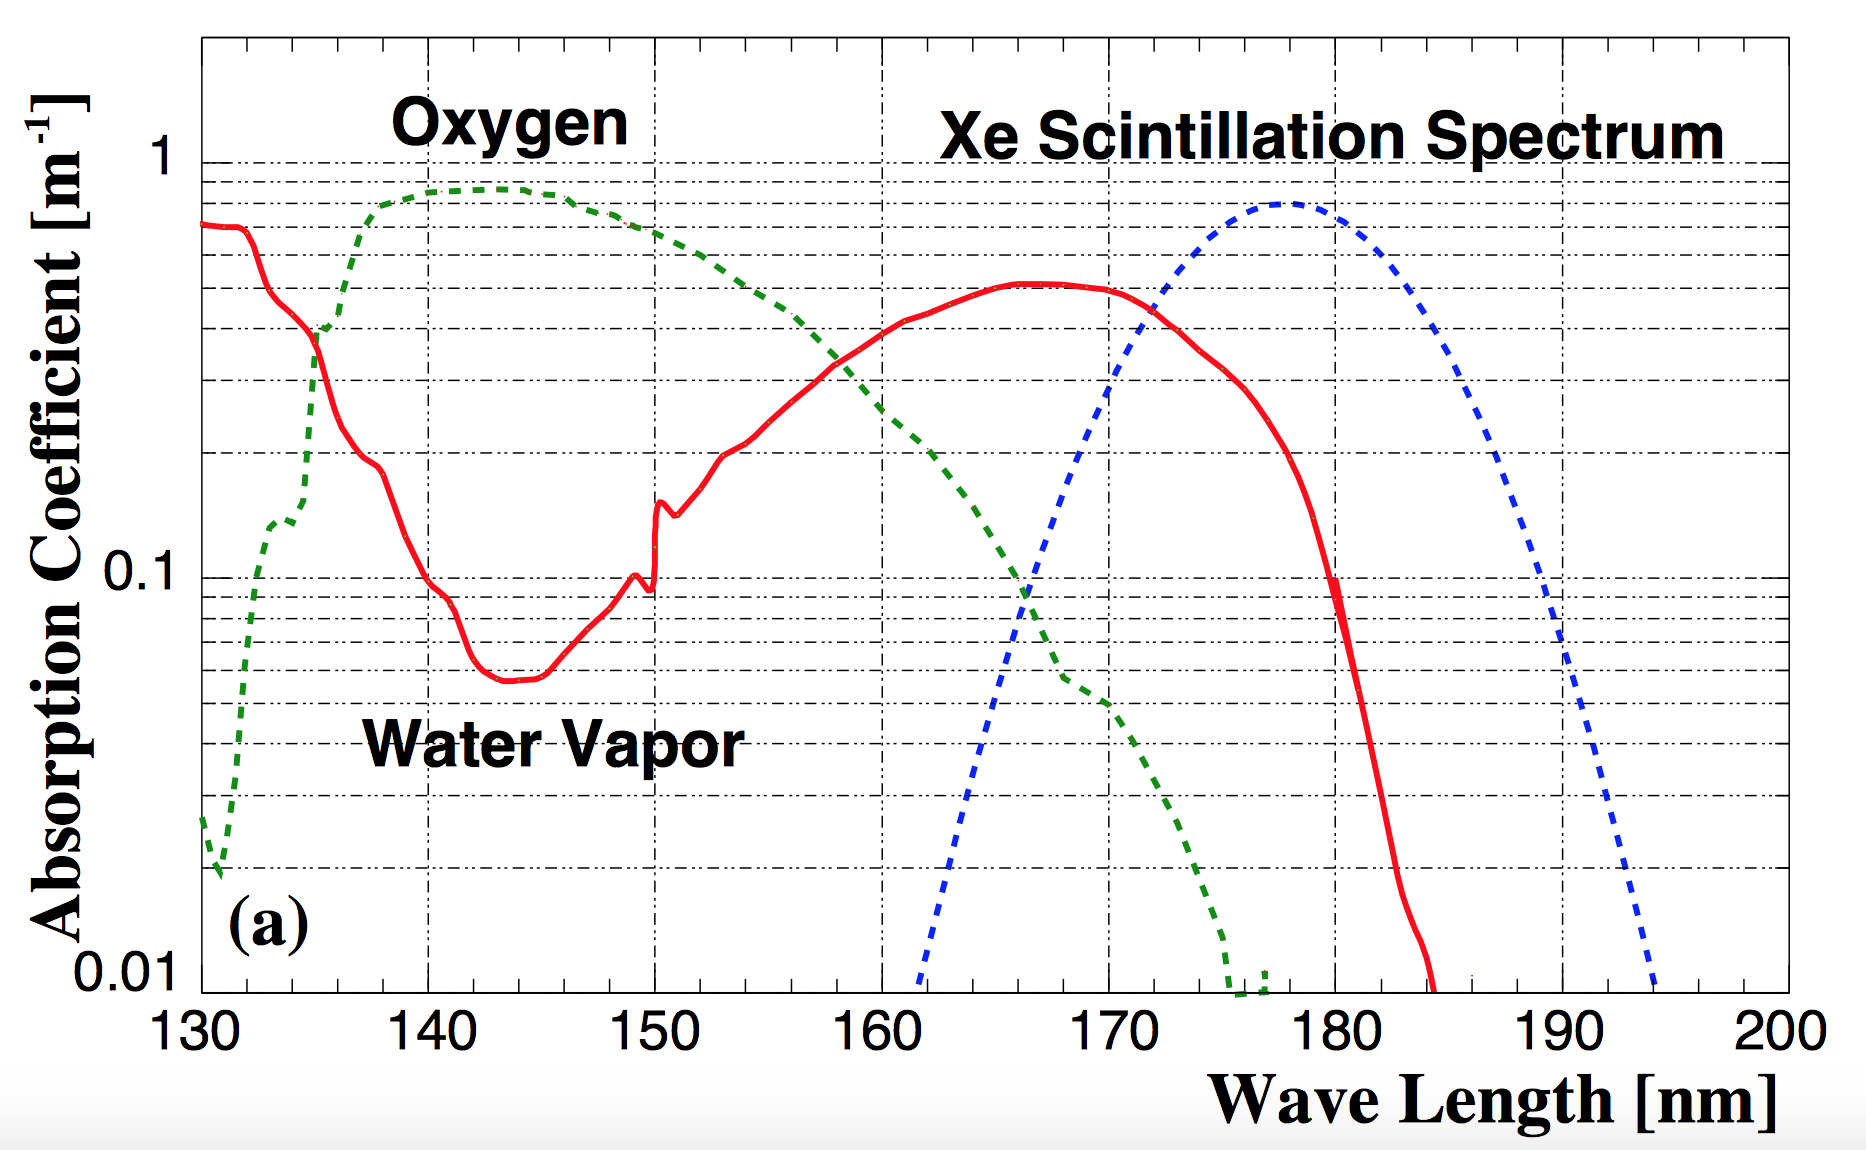
\includegraphics[width=0.8\textwidth]{AbsorptionSpectra}
\caption{Absorption coefficient for photons at 1 ppm \ce{H_2O} vapor (solid red) and \ce{O_2} (dashed green).  The Xe scintillation
spectrum is overlaid for comparison (dashed blue).  \ce{H_2O} impacts Xe scintillation considerably
more than \ce{O_2}.  Image credit: \citeref{Ozone2005}, \ce{H_2O} data from \citeref{Yoshino1996}.}
\label{fig:importance_procedure_effects_photons_absorption_coefficents}
\end{figure}

The relative intensities for different \ce{H_2O}/Xe and \ce{O_2}/Xe concentrations from $0 \mdash 60\ \mathrm{cm}$ are shown in
\figref{fig:importance_procedure_effects_photons_absorption_distance}.  We see that at the level of $\mathcal{O}(100)\ \mathrm{ppb}$ of
oxygen $I / I_0 > 0.8$ at 60 cm.  The effect of water is substantially worse with $I / I_0 < 0.3$, highlighting the necessity of
significant reduction in XENON1T.  Even with a LXe purity that is appreciably better than
\figref{fig:importance_procedure_effects_photons_absorption_distance} $\lambda_{\mathrm{att}} \sim \lambda_{\mathrm{abs}}$ since
the effects of scattering are subdominant with respect to absorption.

\begin{figure}
\centering
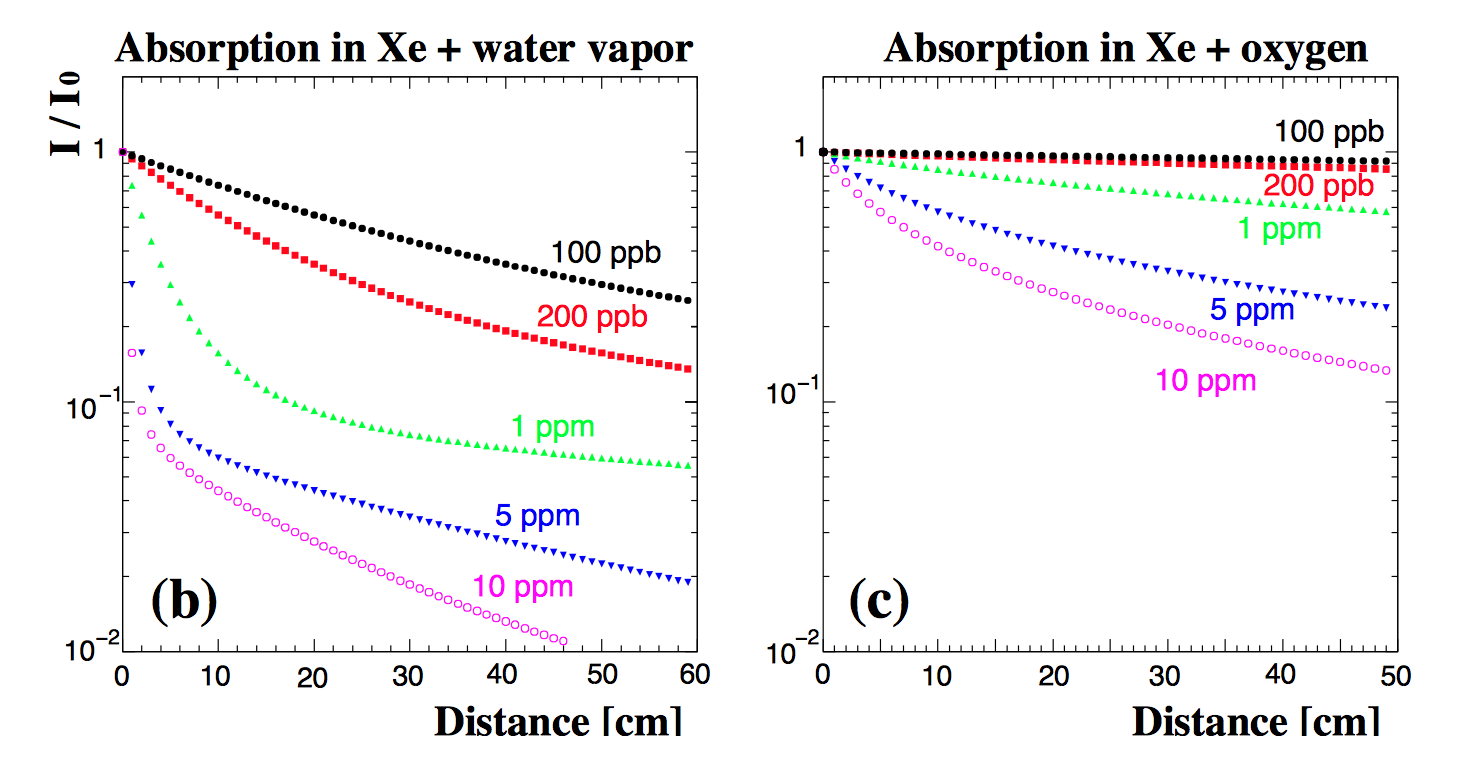
\includegraphics[width=\textwidth]{AbsorptionWithDistance}
\caption{Fraction of initial intensity of xenon scintillation with distance for various concentrations of \htwoo (left) and \otwo
(right).  Image credit: \citeref{Ozone2005}.}
\label{fig:importance_procedure_effects_photons_absorption_distance}
\end{figure}

Photon attenuation ultimately increases our energy threshold as we are less sensitive to lower energies as few photons are
measured.



\subsubsection{Charge Depletion}
\label{subsubsec:importance_procedure_effects_charge}
Electrons that do not recombine will drift antiparallel to $E_d$ in an electron cloud.  As the electron cloud drifts it diffuses both
longitudinally (in the direction of $E_{d}$) and transversely (perpendicular to $E_{d}$).  The
diffusion coefficients $D_{L}$ and $D_{T}$ are dependent on the electric field with $D_{T}/D_{L} \sim 10$.  The electron spread can
be written as $\sigma_{D_{T}} = \sqrt{D_{T} t_{d}}$ where $t_{d} = d/v_{d}$ is the drift time and $d$ is the drift distance.

The behavior of electrons can be classified according to their mobility in the limit of $E \rightarrow 0$, $\mu_0$.  When LXe is
polarized by electrons its high polarizability ($\4.0 \times 10^{-24}\ \mathrm{cm^3}$, highest for noble gas) will both make it
attractive to \electron and interact with nearby Xe atoms through dipole-dipole interaction.  The equilibrium of these two effects
determines the potential energy of the ground state of electrons $V_0$, which is anti-correlated with $\mu_0$.  For LXe these have
been measured to be $V_0 = -0.61 \pm 0.05\ \mathrm{K}$ (\citeref{Tauchert1977}) and $\mu_0 = 2200 \pm 200\ \mathrm{cm^2\ V^{-1}\ s^{-1}}$
(\citeref{Yoshino1976}) at $165\ \mathrm{K}$ (in addition $\mu_0$ was found to be $1900$ and $2200\ \mathrm{cm^2\ V^{-1}\ s^{-1}}$
at $163\mathrm{K}$ by \citeref{Yoshino1976} and \citeref{Miller1968}, respectively).  The large electron mobilities indicate the
electrons are \textit{quasifree}, and have drift velocities that can exceed even those of GXe, as shown in
\figref{fig:importance_procedure_effects_charge_drift_velocity}.

\begin{figure}
\centering
\includegraphics[width=\textwidth]{drift_velocity_field}
\caption{Drift velocity (defined as $W$ here) dependence on reduced electric field $E/N$ where $N$ is the number of molecules per
volume.  Points are from experimental data (\citeref{Gushchin1982, Huang1978, Wagner1967, Pack1992}) and curves are from
calculations.  $1\ \mathrm{Td} = 10^-17\ \mathrm{V\ cm^2}$.  LXe has a higher drift velocity than GXe at
$E/N \lesssim 1\ \mathrm{Td}\ (1\ \mathrm{Td} = 10^{-17}\ \mathrm{V\ cm^2})$.  Image credit: \citeref{Atrazhev2005}.}
\label{fig:importance_procedure_effects_charge_drift_velocity}
\end{figure}

Ions exhibit significantly lower mobility than electrons.  It is parameterized as $\mu \approx \eta^{-\alpha}$ where $\eta$ is the
liquid viscosity and $\alpha = 1 \mdash 2$.  The diffusion coefficients can be calculated with the Nernst-Einstein equation

\begin{equation}
\frac{e D(E)}{\mu (E)} = \mathcal{F} <E>
\end{equation}

\noindent where $\mathcal{F} = 0.5 \mdash 1$ is depends on the electron distribution function (e.g. $\mathcal{F} = 2/3$ for a
Maxwellian distribution).

The mobilities for holes, \ce{TMSi^+}, \ce{O_2^-}, \ce{^{226}Th}, \ce{^{208}Tl}, and \ce{Xe_2^+} in in LXe are listed in
\tabref{tab:importance_procedure_effects_charge_mobilities}.  They are ${\sim} 10^6$ times smaller than the electron mobility.

\begin{table}
\centering
\begin{tabular}{cccccc}
\hline
Ion & T [K] & $\mu\ [10^{-4}\ cm^2\ V^{-1}\ s^{-1}]$ & Ref, \\
\hline
holes & 161 & 35 & \citeref{Hilt1994b} \\
holes & 230 & 46 & \citeref{Hilt1994b} \\
\ce{TMSi^+} & 162 & 2 & \citeref{Hilt1994a} \\
\ce{TMSi^+} & 192 & 3 & \citeref{Hilt1994a} \\
\ce{O_2^-} & 162 & 6 & \citeref{Hilt1994a} \\
\ce{O_2^-} & 192 & 10 & \citeref{Hilt1994a} \\
\ce{^{226}Th^+} & 162 & 2.4 & \citeref{Wamba2005} \\
\ce{^{208}Tl^+} & 163 & 1.33 & \citeref{Walters2003} \\
\ce{Xe_2^+} & 184.2 & 2.85 & \citeref{Davis1962} \\
\ce{Xe_2^+} & 192.1 & 3.17 & \citeref{Davis1962} \\
\hline
\end{tabular}
\caption{Ion mobilities in LXe.  All ions listed are positive with the exception of \ce{O_2^-}.  Positive holes have mobilities that are
${\sim} 10$ greater than ions.  Summarized data is given in \citeref{Aprile2006a}.}
\label{tab:importance_procedure_effects_charge_mobilities}
\end{table}

Hole mobility can be described by the hopping model of charge carrier transport.  In this temperature-dependent model charge is
propagated through jumps between traps yielding

\begin{equation}
\mu = \frac{e b^2}{k_{\mathrm{B}} T} \omega
label{eq:importance_procedure_effects_charge_mobility_simple}
\end{equation}

\noindent where $b$ is the average jump distance and $\omega$ is the jumping frequency, parameterized as

\begin{equation}
\omega = P \Big( \frac{\omega_0}{2 \pi} \Big) e^{-E_{\mathrm{a}} / k_{\mathrm{B}} T}
\end{equation}

\noindent where $\omega_0$ is the phonon frequency, $P(\omega_0 / 2 \pi)$ is the tunneling probability between adjacent holes with
activation energy $E_{\mathrm{a}}$.  \figref{importance_procedure_effects_charge_hole_mobility} shows hole mobility in
LXe.  The solid curve represents a model that parameterizes \eqref{eq:importance_procedure_effects_charge_mobility_simple} as

\begin{equation}
b^3(T) = \sqrt{2} M / \rho (T)
\end{equation}

\noindent where $M$ is the atomic mass of xenon and $\rho (T)$ is the temperature-dependent density (\citeref{Hilt1994b}).  It
additionally assumes the hole is self-trapped between two rare atoms in a potential well, forming a polaron.  It gives a hole mobility of

\begin{equation}
\mu (T) = \frac{e b^2 (T)}{k_{\mathrm{B}}} \frac{2 \pi}{h} \sqrt{\frac{\pi}{4 E_a k_{\mathrm{B}} T}} J_0^2
e^{-2 \alpha b(T)} e^{-E_a / k_{\mathrm{B}} T}
\label{eq:importance_procedure_effects_charge_mobility_polaron}
\end{equation}

\noindent where $h$ is Planck's constant and and $J(T) = J_0 e^{-\alpha b(t)}$ is the transfer integral.

\begin{figure}
\centering
\includegraphics[width=0.8\textwidth]{hole_mobility}
\caption{Fig. 3.15 in Aprile book.  Temperature-dependent drift mobility for holes in LXe.  Data is shown as empty triangles.  A fit
using \eqref{eq:importance_procedure_effects_charge_mobility_polaron} is shown as the solid line.  Image credit: \citeref{Aprile2006a}
(redrawn from \citeref{Hilt1994b}.)}
\label{fig:importance_procedure_effects_charge_hole_mobility}
\end{figure}

As the cloud drifts electronegative impurities can bond to \electron and prevent them from reaching the liquid-gas interface, thereby
decreasing proportional scintillation

\begin{equation}
e^{-} + S \rightarrow S^{-}
\label{eq:impurity_attach}
\end{equation}

\noindent where $S$ refers to the impurity (e.g. $e^- + \mathrm{O_2} \rightarrow \mathrm{O_2^-}$).

Electronegative impurities
in particular present a problem
since they attach to drifting $e^{-}$,
lowering the number that reach the liquid-gas interface and thus decreasing the secondary scintillation.  The attachment process
is \eqref{eq:impurity_attach}.


\noindent where $S$ is the impurity.  The number of \electron captured is dependent drift time $t_{d}$ and the
attachment rate of
the impurities $k_{S}$, both of which depend on $E_{d}$.  Clearly then an advantage of larger
\efields is a larger
\vd (up to a point, see \figref{fig:drift_velocity}) and thus less time in the liquid.  Doping LXe with organic materials such as butane
can increase \vd at stronger
\efields but are not used in DM detectors due to difficulty in purifying (\citeref{Yoshino1976}).  The rate at which electrons are
absorbed by impurities is proportional to the number of electrons, impurities, and impurity attachment rate.  Assuming the the density
of impurities in the liquid and $E_{d}$ are uniform we find

In an electric field $E$ an \electron that is freed but does not recombine with its parent or other ionized atoms will move anti-parallel
to the field at drift velocity $v_{d}$.  At fields of $\lesssim 100\ \mathrm{V\ cm^{-1}}$ drift velocity is nearly proportional to
$E$ and is given by $v_{d} = \mu E$
where $\mu$ is the electron mobility.  For this energy region $\mu \sim 2200\ \mathrm{cm^{2}\ V^{-2}\ s^{-1}}$ (\citeref{Yoo2015}).  As
$E$ increases $v_{d} \propto E^{1/2}$ and ultimately flattens at $\sim 3\ \mathrm{mm\ \mu s}$.  \figref{fig:drift_velocity} shows \vd
as a function of $E$ and \tabref{tab:drift_velocity} gives the approximate relationship.

The strength of $E$ affects the number of electrons freed, as a larger field decreases
recombination electron-ion recombination.  In liquid noble gas detectors used for DM searches such a field can be used to drift the
\electron to the surface of the liquid, where they are extracted across a small region of gas.  Doing so will produce secondary
scintillation as the \electron will energize the atoms in the gas, freeing more \electron in turn.  Because the amount of scintillation
produced per electron is independent of the number of electrons extracted this is also known as proportional scintillation.  Thus, by
measuring this scintillation the number of \electron extracted can be determined.  Details of \electron drift and proportional
scintillation is found in \secref{subsec:tpcs_working_principle}.

For $E \lesssim 100\ \mathrm{V\ cm^{-1}}$ \vd$\propto E$, $100 \lesssim E \lesssim 10^{3 \ mdash 4}$
\vd$\propto E^{1/2}$, and $E \gtrsim 10^{4}$ \vd plateaus at $\sim 3\ \mathrm{mm\ \mu s^{-1}}$ (\citeref{Miller1968}).

\begin{table}
 \centering
 \begin{tabular}{cc}
 \hline
 $E$ [V cm$^{-1}$] & \vd [mm $\mu$s$^{-1}$] \\
 \hline
 $\lesssim 100$ & \vd$\propto E$ \\
 $\sim 100 \mdash 10^{3 \mdash 4}$ & \vd$\propto E^{1/2}$ \\
 $\gtrsim 10^{4}$ & \vd$\sim 3$ \\
 \hline
 \caption{Drift velocity \vd dependence on electric field for LXe.}
 \end{tabular}
 \label{tab:drift_velocity}
\end{table}

\begin{figure}
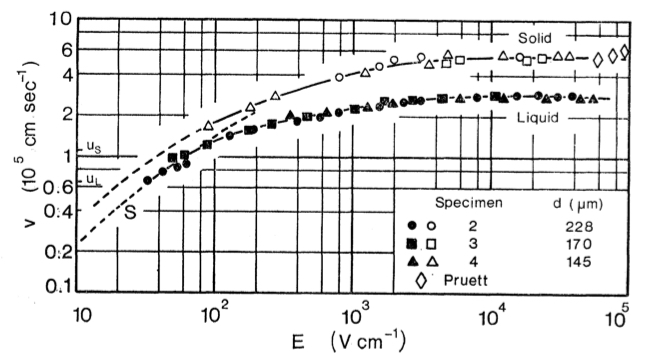
\includegraphics[angle=0.5, width=0.8\textwidth]{DriftVelocity}
\caption{Drift velocity for solid and liquid xenon}
\label{fig:drift_velocity}
\end{figure}
In addition to absorbing VUV photons impurities can attach to drifting electrons.






Page 257 in Aprile book